\documentclass[margin=0px]{article}

\usepackage{listings}
\usepackage[utf8]{inputenc}
\usepackage{graphicx}
\usepackage{float}
\usepackage[a4paper, margin=0.7in]{geometry}
\usepackage{amsthm}
\usepackage{fancyhdr}
\usepackage{setspace}

\onehalfspacing

\renewcommand{\figurename}{ábra}
\newenvironment{tetel}[1]{\paragraph{#1 \\}}{}

\pagestyle{fancy}
\lhead{\it{PTI BSc Záróvizsga tételek}}
\rhead{8. Objektumelvű modellezés}

\title{\textbf{{\Large ELTE IK - Programtervező Informatikus BSc} \vspace{0.2cm} \\ {\huge Záróvizsga tételek}} \vspace{0.3cm} \\ 8. Objektumelvű modellezés}
\author{}
\date{}

\begin{document}
\maketitle

\begin{tetel}{Objektumelvű modellezés}
    Az objektumelvű modellezés nézetrendszerei: statikus modell (osztálydiagram, objektumdiagram, csomag diagram, komponens diagram); dinamikus modell (állapotgép diagram, szekvencia diagram, kommunikációs diagram, használati eset diagram).
\end{tetel}

\section{Az objektumelvű modellezés nézetrendszerei}

\textbf{Objektumelvű programozás} = adatabsztrakció + absztrakt adattípus + típusöröklődés
\begin{itemize}
    \item Absztrakció

          Programozás adott szintjén a megoldás szempontjából
          lényegtelen részletek elhanyagolása.

    \item Adattípus

          Az adattípus egy $ (A,F) $ rendezett pár, ahol $ A $ az adatok halmaza $ F $ pedig a műveletek véges halmaza. ($ \forall f \in F : f:A^n \rightarrow A $) Létezik egyszerű és összetett adattípus.\\
          \textbf{Típusosztály:} A típus komplex leírása, mely az adott adattípus \underline{absztrakt} (PAR + EXP) és \underline{konkrét} (IMP + BODY) leírását szolgálja. Tehát:\\\\
          Típusosztály = (PAR, EXP, IMP, BODY), ahol:\\
          PAR = \textless paraméterek tulajdonságai \textgreater\\
          EXP = \textless típusobjektumok halmaza és műveltei neve, szintaktikája, szemantikája \textgreater\\
          IMP = \textless más osztályból átvett szolgáltatások \textgreater\\
          BODY = \textless típusosztály ábrázolása, megvalósítása \textgreater\\

    \item Típusöröklődés

          A típusöröklődés két fő formája: \textit{specializáció} és  \textit{újrafelhasználás}
          \begin{enumerate}
              \item A subclass átveszi az absztakt tulajdonságokat és azt az export részben használja fel
              \item Típushalmaz, paraméterhalmazok, műveletek nevei átdefiniálódhatnak.
              \item subclass típushalmaza = superclass típushalmaza
          \end{enumerate}

          A specializáció következményei:
          \begin{itemize}
              \item polimorfizmus

                    Minden változónak két típusa van: \textit{statikus} (deklaráció során kapott) és \textit{dinamikus} (deklaráció pillanatában megegyezik a statikussal, de később megváltozhat, ha egy superclass példánynak adunk értékül egy subclass példányt)
              \item dinamikus kötés

                    A dinamikus típusnak megfelelő kiszámítási szabály hozzárendelése a függvényhez attribútumhoz, a végrehajtás pillanatában
          \end{itemize}
          \paragraph{Nézetrendszerek}
          \begin{itemize}
              \item használati szempont

                    Kinek nyújt a rendszer szolgáltatást? (Személyek vagy más rendszerek, programok)

              \item Szerkezetei strukturális, statikus szempont

                    Milyen egységek vannak, ezeknek mi a feladata, és hogyan kapcsolódnak egymáshoz?

              \item Dinamikus szempont

                    Az egyes részegységek hogyan viselkednek, milyen állapotokat vesznek fel, azokat milyen események hatására váltják? Milyen az egységek között együttműködés mechanizmusa? Időben hogyan játszódnak le közöttük az üzentek?

              \item Implementációs szempont

                    Milyen szoftverkomponensek, és azok között milyen kapcsolatok vannak?

              \item Környezeti szempont

                    A rendszer milyen hardver és szoftver erőforrást igényel a megoldás során?
          \end{itemize}
\end{itemize}
\section{Statikus modell (osztálydiagram, objektumdiagram, csomag diagram, komponens diagram)}
\subsection{Osztáldiagram}
A megoldás szerkezetét leíró összefüggő gráf, melynek csomópontjaihoz az osztályokat, éleihez pedig az osztályok közötti relációkat (öröklődés, asszociáció, aggregáció, kompozíció) rendeljük.

\noindent
A rendszerhez csak egy osztálydiagram tartozik.

\begin{description}
    \item[Osztályok] \hfill \\

        Egy osztály a következőképp néz ki:
        \begin{figure}[H]
            \centering
            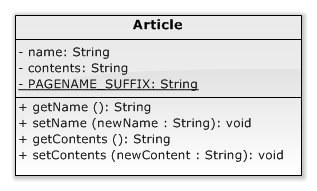
\includegraphics[width=0.4\textwidth]{img/osztaly.png}
            \caption{Osztály}
        \end{figure}

        Az osztályt leíró téglalap 3 részre van osztva.
        \begin{itemize}
            \item Az első részbe az osztály neve kerül.

                  Ha az osztály absztrakt, a nevét dőlt betűvel írjuk.

            \item A második részbe az osztály attribútumai kerülnek.

                  Az attribútum formátuma: \textit{Attribútumnév : Típus}
                  A statikusságot aláhúzással jelöljük.
                  Az attribútumok láthatóságát is fel lehet tüntetni: \textit{ publikus (+), privát (-), védett (\#)}

            \item A harmadik részbe az osztály metódusai kerülnek.

                  A metódusok formátuma: \textit{Metódusnév(Paraméterlista):Visszatérési érték}, ahol a paraméterlista \textit{Paraméternév:Típus} fomrátumú paraméterekből áll.
                  Absztraktságot, statikusságot, és láthatóságot az előzőekben leírtakkal azonosan jelöljük.
        \end{itemize}
    \item[Osztályok közötti kapcsolatok:] \hfill \\

        \begin{itemize}
            \item öröklődés

                  Két osztály közötti absztrakciós kapcsolatot jelöl
                  \begin{figure}[H]
                      \centering
                      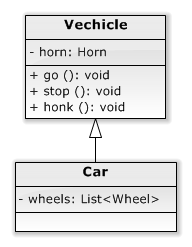
\includegraphics[width=0.2\textwidth]{img/oroklodes.png}
                      \caption{Öröklődés}
                  \end{figure}

            \item asszociáció

                  Ez a legáltalánosabb reláció két osztály között. Az asszociáció két osztály
                  közötti absztrakt reláció, amely kétirányú társítást fejez ki. A
                  reláció absztrakt volta azt jelenti, hogy a reláció konkretizálása osztályok
                  objektumainak összekapcsolásában valósul meg.

                  Az asszociációnak lehet:
                  \begin{itemize}
                      \item Neve, azonosítója
                      \item Iránya
                      \item Multiplicitása

                            Akár egy érték, akár intervallum. A * szimbólum kitüntett szerepet kap, jelentése: bármennyi, akár nulla is. (Pl: 3, 1..4, 5..*, *)
                      \item Szerepe
                      \item Navigálhatósága

                            A társított osztályok közül csak az egyik ismeri a másikat. (Ha nem tüntetjük fel, kölcsönös elérhetőséget feltételezünk)

                            \begin{figure}[H]
                                \centering
                                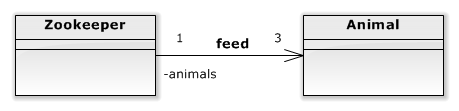
\includegraphics[width=0.5\textwidth]{img/asszociacio.png}
                                \caption{Asszociáció}
                            \end{figure}
                  \end{itemize}
            \item aggregáció

                  Az aggregáció egy speciális asszociáció, mely egész-rész kapcsolatot fejez ki. Azonban ha két osztály között aggregációs reláció áll fenn, a két osztály objektumai egymástól függetlenül is létezhetnek (Ezt un. laza tartalmazási relációnak nevezik) A relációt jellemzi ezen kívül a tranzitivitás, és a közös attribútumok illetve szolgáltatások. Különböző aggregátumoknak lehetnek közös komponenseik.
                  \begin{figure}[H]
                      \centering
                      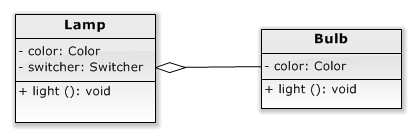
\includegraphics[width=0.5\textwidth]{img/aggregacio.png}
                      \caption{Aggregáció}
                  \end{figure}
            \item kompozíció

                  A kompozíció egy speciális aggregáció, mely \textit{fizikai} tartalmazást jelöl. Nem jellemzi többé az objektumok független létezése, a két objektum egyszerre jön létre és szűnik meg. Tehát a tartalmazó objektumnak gondoskodnia kell a tartalmazott létrehozásáról és megszüntetéséről. Egy komponens legfeljebb egy tartalmazó \underline{objektumhoz} tartozhat. A kompozíciós kapcsolat és az attribútum jellegű kapcsolat két objektum között szemantikailag azonos.
                  \begin{figure}[H]
                      \centering
                      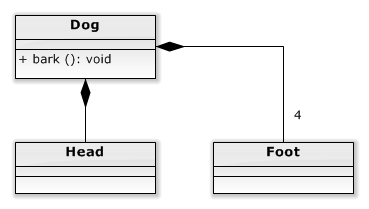
\includegraphics[width=0.4\textwidth]{img/kompozicio.png}
                      \caption{Kompozíció}
                  \end{figure}
        \end{itemize}
\end{description}

\subsection{Objektumdiagram}
Az objektumdiagram egyszeresen összefüggő gráf, amelynek csomópontjaihoz az objektumokat, éleihez pedig az objektumok közötti összekapcsolásokat rendeljük.

A rendszerhez különböző időpillanatokban más-más objektumdiagram tartozhat. (Viszont mindegyiknek meg kell felelnie az osztálydiagramnak)

\begin{description}
    \item[Objektumok] \hfill \\
        Az objektumokat az osztályokhoz hasonlóan egy téglalap írja le. Egy ilyen téglalapnak két része van. Az első részben az objektum neve (opcionális) és típusa található a következő formátumban: \textit{Objektumnév : Típus}, melyet aláhúzással tarkítunk. A második részbe az objektum attribútumai és azok értékei kerülhetnek, a következő formátumban: \textit{Attribútumnév=érték}.
        \begin{figure}[H]
            \centering
            \includegraphics[width=0.2\textwidth]{img/objektum.png}
            \caption{Objektum}
        \end{figure}
    \item[Objektumok közötti kapcsolatok] \hfill \\
        Az objektumokat összekötő relációk az osztálydiagramon lévőkkel megegyezőek (Öröklődésnek ezen a szinten nincs értelme):
        \begin{itemize}
            \item asszociáció
                  \begin{figure}[H]
                      \centering
                      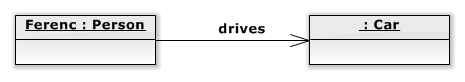
\includegraphics[width=0.5\textwidth]{img/asszociacio2.png}
                      \caption{Asszociáció}
                  \end{figure}
            \item aggregáció
                  \begin{figure}[H]
                      \centering
                      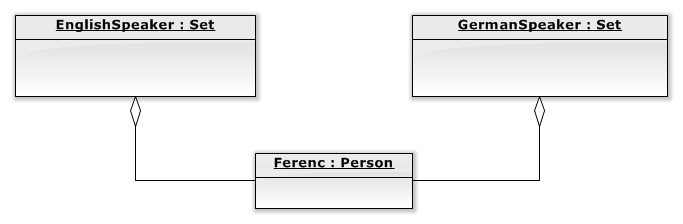
\includegraphics[width=0.7\textwidth]{img/aggregacio2.png}
                      \caption{Aggregáció}
                  \end{figure}
            \item kompozíció
                  \begin{figure}[H]
                      \centering
                      \includegraphics[width=0.5\textwidth]{img/kompozicio2.png}
                      \caption{Aggregáció}
                  \end{figure}
        \end{itemize}
\end{description}

\subsection{Csomag diagram}
A csomag diagram alapvetően más modell elemek csoportosítására használható, és mint ilyen, szintén minden fejlesztési fázisban használatos. A használati eset modell elkészítése során a használati eset leltár esetén már említésre került, ebben a fejezetben összefoglaljuk a részletes szabályokat. A csomag jele az UML-ben egy ``füles'' téglalap. A fül felirata lehet a csomag neve, de írható a téglalapba is. A csomagnév fölött sztereotípiát adhatunk meg, alatta megszorítást. A csomag tartalma lehet bármilyen szövegesen vagy diagrammal megadott modell elem, illetve azok halmaza. A korábban már említett használati eset leltár például használati eseteket tartalmazó csomagokból áll. A csomagok újabb csomagot is tartalmazhatnak. Egy modell elem csak egy csomaghoz tartozhat. Így a csomagok fa struktúrájú hierarchiát alkotnak, hasonlóan, mint a filerendszerek elemei, vagy a Java csomagok.

A <<system>> sztereotípiával jelzett csomag a legfelső szintű, az egész alkalmazást jelképező csomag. A csomagok közötti függőségek szaggatott,  nyitott hegyű nyíllal ábrázolhatjuk. A kapcsolat jellegét sztereotípiával pontosíthatjuk. Az UML csomag egyben egy névteret is képvisel, ezért egy csomagon belül nem lehet két azonos nevű modell elem. Ha egy másik csomagban levő modell elemre akarunk hivatkozni, azt a minősített nevével tehetjük meg. A minősített név tartalmazza azon csomagok neveit, amelyeken keresztül eljuthatunk az adott modell elemig. A csomagneveket a :: választja el egymástól.

A csomag elemeihez public(+) és private (-) láthatóságot is rendelhetünk, hasonlóan az osztályok elemeihez.
A minősített névvel való hivatkozás nehézkes lehet a hosszúsága miatt, és minden ilyen hivatkozásra hatással lehet a csomagok átszervezése. Ezért helyette egyszerűbb és célszerűbb a csomagok közötti hivatkozásokat a függőséget jelölő (szaggatott vonallal rajzolt) nyíllal és sztereotípiákkal jelölni (importálás). Az importált elem az importáló csomag számára látható lesz. A használható sztereotípiák:

<<import>>: nyilvános import, az importáló csomag tovább exportálhatja

<<access>>: privát import, csak az importáló csomag láthatja.

Jelölése:
\begin{itemize}
    \item Az importáló csomagtól közvetlenül az importált elemre mutató szaggatott nyíl
    \item Az importáló csomagtól az importált elemet tartalmazó csomagra mutató nyíl, a sztereotípia után írva az importálandó elem neve
    \item A két csomag között rajzolt, elemnév nélküli nyíl a teljes csomag valamennyi elemének importálását jelenti.
\end{itemize}

\begin{figure}[H]
    \centering
    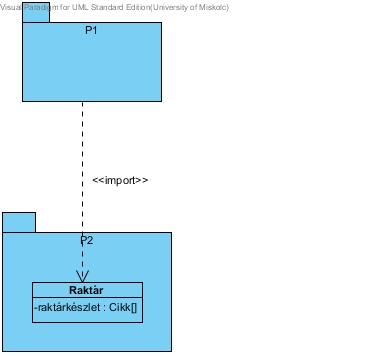
\includegraphics[width=0.5\textwidth]{img/csomag_diagram.jpg}
    \caption{Csomag diagram: elem importálása}
\end{figure}

\subsection{Komponens diagram}
A komponens az UML-ben egy olyan univerzális egység, amely valamilyen szolgáltatás halmazt képvisel, azokat egy egységbe zárja. A szolgáltatásokat más komponensek interfészeken keresztül érhetik el. Egy komponens kicserélhető egy másikkal, ha ugyanolyan interfésszel rendelkezik, és ugyanazokat a szolgáltatásokat nyújtja.

Egy komponens tartalmazhat más komponenseket.

A komponensek fogalma jól használható a fejlesztés minden fázisában. Így jelenthet egy implementációs értelemben vett komponenst (például egy Enterprise JavaBean-t), de akár egy komplett alrendszert is (például könyvelés).

A komponens jele egy téglalap a <<component>> sztereotípiával, vagy egy ikonnal megjelölve. A komponens a külvilággal csatlakozókon (port) keresztül teremt kapcsolatot. Minden csatlakozóhoz egy vagy több interfész kapcsolható. A külvilág felé szolgáltatásokat nyújtó interfészt (nyújtott interfész) egy körrel, a komponens által másoktól igényeltet (megkövetelt interfész) egy félkörrel jelöljük. A komponensek közötti kapcsolatokat az interfészek összeillesztésével ábrázolhatjuk. Egy nyújtott interfész csak egy megkövetelt interfésszel állhat kapcsolatban. (Ezt jól szemléltetik a jelölések is.)

A komponens diagram jelöléseit szemlélteti az alábbi ábra, amely az esettanulmány komponens diagramjának egy részlete.

\begin{figure}[H]
    \centering
    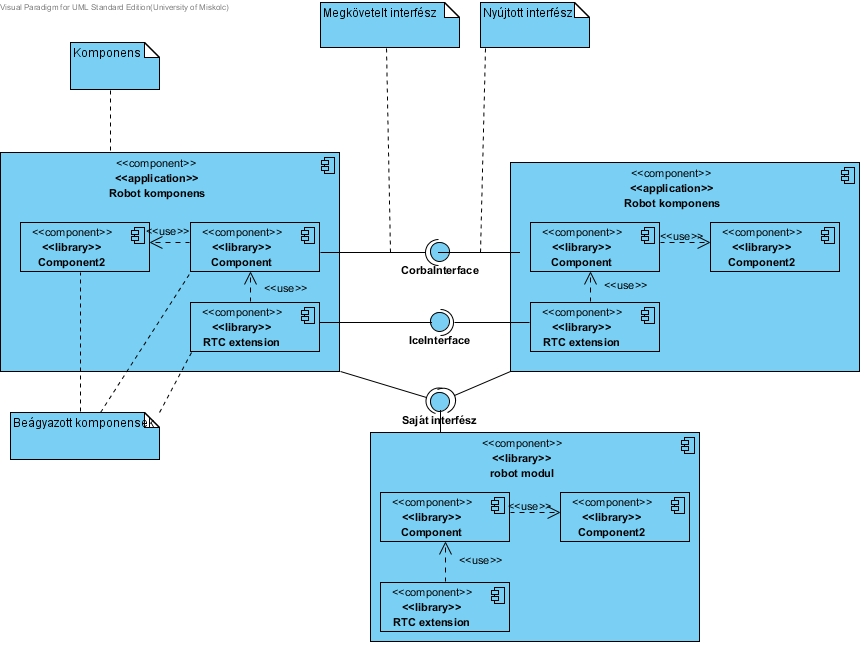
\includegraphics[width=0.5\textwidth]{img/komponens_diagram.jpg}
    \caption{Komponens diagram}
\end{figure}


\section{Dinamikus modell (állapotdiagram, szekvenciadiagram,\\ együttműködési diagram, tevékenységdiagram)}

\subsection{Állapotdiagram}
Az állapotdiagram egy összefüggő irányított gráf, amelynek csomópontjaihoz az állapotokat rendeljük, éleihez pedig az eseményeket. (Két csúcs között több állapotátmenetet is jelölhetünk, hiszen több esemény hatására is létrejöhet)
\begin{description}
    \item[Állapot] \hfill \\
        Az objektum állapotát az attribútumok konkrét értékeinek n-esével jellemezzük.

        Az állapotnak van azonosítója, mely legtöbbször az állapot neve (de lehet maga az invariáns, vagy az attribútumok konkrét értéke). Az állapotot esemény hozza létre és szünteti meg. Az állapot mindaddig fennmarad, míg az attribútumok kielégítik az állapotot leíró invariánst. Az állapotot egy lekerekített téglalappal jelöljük, melyben az azonosítót tüntetjük fel.

        Speciális (rendszeren kívüli) állapotok: Kezdőállapot, Végállapot
    \item[Esemény] \hfill \\
        Eseménynek nevezzük azt a tevékenységet, történést, amely valamely objektum állapotát megváltoztatja.

        Az esemény lehet paraméteres vagy paraméter nélküli, és lehet előfeltétele. Az események között sorrendiség áll fent, így egy esemény lehet megelőző eseménye. Egy eseményt a következőképp írhatunk le:\\
        \textless esemény \textgreater (\textless paraméterek\textgreater)[\textless feltétel\textgreater]/\textless megelőző esemény\textgreater

        Az eseményeket az állapotok közötti állapotátmenetekre írjuk.
        \begin{figure}[H]
            \centering
            \includegraphics[width=0.5\textwidth]{img/plane.png}
            \caption{Repülőgép állapotgépe}
        \end{figure}
\end{description}
\subsection{Szekvenciadiagram}
A szekvencia diagram az objektumok közötti üzenetváltások időbeli menetét
szemlélteti.
\begin{description}
    \item[Osztályszerep] \hfill \\
        Az osztály szerepét olyan egy vagy több objektum testesíti meg, melyek az üzenetküldés szempontjából konform módon viselkednek.
    \item[Osztályszerep életvonal] \hfill \\
        Az életvonal az osztályszerep időben való létezését jelenti.
        \begin{figure}[H]
            \centering
            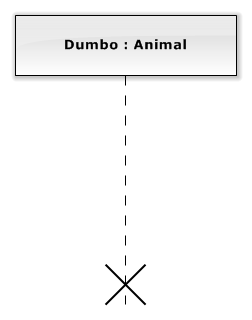
\includegraphics[width=0.3\textwidth]{img/eletvonal.png}
            \caption{Életvonal}
        \end{figure}
    \item[Aktivációs életvonal] \hfill \\
        Az aktivációs életvonal azt az állapotot jelenti, amikor az osztályszerep megtestesítői műveleteket hajtanak végre, vagy más objektumok vezérlése alatt állnak.
        \begin{figure}[H]
            \centering
            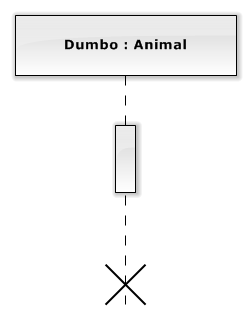
\includegraphics[width=0.3\textwidth]{img/aktivacios_eletvonal.png}
            \caption{Aktivációs életvonal}
        \end{figure}
    \item[Üzenet] \hfill \\
        Az üzenet az objektumok közötti információátadás formája. Az üzenet küldésének az a célja, hogy az objektum működésbe hozza a másik objektumot. Az üzenet azok között az objektumok között jöhet létre, amelyek az objektumdiagramban kapcsolatban állnak. Az üzenetnek van azonosítója (neve, szövege), lehet paramétere, sorszáma.

\end{description}
\subsection{Együttműködési diagram}
Az együttműködési diagram azt hivatott bemutatni, hogy miként működnek együtt az osztályok objektumai, milyen üzenetek cseréje révén valósul meg ez az együttműködés.
(Csak azok az objektumok relevánsak, amelyek osztályait az osztálydiagramban asszociációs kapcsolat köt össze. A diagram mutatja ezt az összekapcsolást és az ehhez tartozó
üzenetváltásokat, ezért az együttműködési diagram az objektumdiagram bizonyos értelemben vett kiterjesztésének tekinthető.)

Az üzenet küldését egy nyíl mutatja, amely az asszociáció mellett kap helyet és a címzett irányába mutat. Az üzenet azonosítója a nyíl mentén helyezkedik el. Az üzenetnek lehet argumentuma és eredménye. Ezeket egy kis körből induló nyíl mellett helyezzük el, ahol a nyíl az információ áramlásának irányát mutatja.


\subsection{Tevékenységdiagram}
A tevékenységdiagram (aktivációs diagram) a probléma megoldásának lépéseit szemlélteti, a párhuzamosan zajló vezérlési folyamatokkal együtt.

Ha egy tevékenységet
egy másik tevékenység követ közvetlenül, akkor a két tevékenységet
nyíllal kötjük össze. Ha adatot (objektumot) ad át egy tevékenység
egy másik tevékenységnek, akkor a küldő tevékenységből szaggatott
nyíl vezet az objektumot reprezentáló téglalaphoz, és a téglalaptól
szaggatott nyíl mutat a fogadó tevékenységre. A téglalapban szögletes
zárójelek között megadhatjuk az objektum állapotát, státuszát is.
\begin{figure}[H]
    \centering
    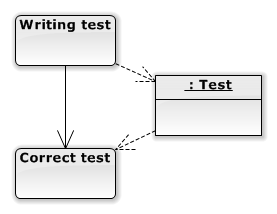
\includegraphics[width=0.3\textwidth]{img/tevekenyseg.png}
    \caption{Objektum átadás}
\end{figure}

Lehetőség van arra, hogy bizonyos feltételek teljesülése esetén eltérő
tevékenységeket hajtsunk végre, illetve tevékenységek végrehajtását
feltételekhez kössük. Ekkor egy rombuszt kell elhelyeznünk a diagramban,
amelyből kivezető nyilakra írjuk a feltételeket.

\begin{figure}[H]
    \centering
    \includegraphics[width=0.4\textwidth]{img/tevekenyseg2.png}
    \caption{Feltétel ábrázolása}
\end{figure}

\subsection{Kommunikációs diagram}

A kommunikációs diagram, a szekvencia diagramhoz hasonlóan, objektumok közötti üzenetváltásokat képes ábrázolni, azonban ebben az esetben nem az üzenetváltások időbeliségére helyezzük a hangsúlyt, hanem az üzenetváltásokban részvevő objektumok közötti kapcsolatokra. A szekvencia diagramon az objektumok kapcsolata csak közvetve jelenik meg, azáltal, hogy mely elemek között van interakció. A kommunikációs diagramon az együttműködő objektumok az osztálydiagramoknál már megismert, asszociációkat jelző vonalakkal (nyilakkal) vannak összekötve. Az üzenetek időbeli sorrendjét az üzeneteket számozása jelzi.

A kommunikációs diagramon is szerepelhet aktor, mint az üzenet forrása vagy címzettje.

Jelölni lehet, ha egy objektum aktív (önállóan képes üzenetet küldeni), illetve ha egy üzenet nem egy objektumhoz, hanem azonos osztályhoz tartozó objektumok egy halmazához irányul (multiobjektum).

Példaként rajzoljuk meg egy bank automatából való készpénzfelvétel kommunikációs diagramját. Feltételezzük, hogy az ügyfél a kártya beolvasásával és a PIN lód megadásával már azonosította magát, és a lehetséges funkciók közül kiválasztotta a készpénzfelvételt.

\begin{figure}[H]
    \centering
    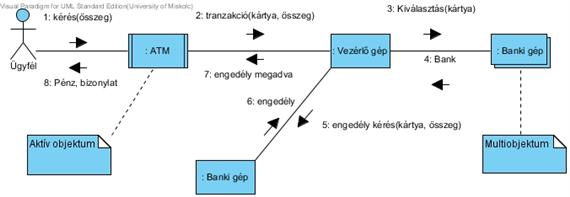
\includegraphics[width=0.4\textwidth]{img/kommunikacios_diagram.jpg}
    \caption{Kommunikációs diagram}
\end{figure}

\section{Használati esetek diagramja}
A használati esetek diagramja a felhasználók szempontjából kívánja
szemléltetni azt, hogy a rendszer miként működik, függetlenül attól,
hogy a szolgáltatásait hogyan valósítja meg.

\noindent
A diagram részei:
\begin{itemize}
    \item használati esetek
    \item felhasználók
    \item felhasználási relációk
\end{itemize}

A használati esetek a rendszer funkcióinak összefoglalásai, szolgáltatási
egységek. Ez az egység az akcióknak egy olyan sorozata, amelyekkel
a rendszer a felhasználók egy csoportjával működik együtt.

A használati esetet egy ovális alakzattal jelöljük. A használati eseteket téglalapba foglaljuk, ez jelzi a rendszer határait.

A felhasználók az adott rendszeren kívüli egységek, más programrendszerek,
alrendszerek, osztályok, illetve személyek lehetnek. Ezek
aktor szerepet töltenek be. A diagramon egy pálcikaember figurával jelöljük.

A felhasználási relációk kapcsolják össze a használati eseteket a
felhasználókkal. A relációk egymással is kapcsolatban állhatnak, amit
a diagramban fel lehet tüntetni. A lehetséges relációk a következők:
\begin{itemize}
    \item asszociáció \\
          Egy felhasználó és egy használati eset közötti kapcsolatot jelez. (Egyszerű vonal)
    \item általánosítás \\
          Az egyik használati eset a másik általánosabb formája. (Egyszerű vonal, végén fehér háromszöggel)
    \item kiterjesztés \\
          Az egyik használati eset a másikat terjeszti ki. Ennek
          során viselkedéseket illeszt be megadott beszúrási pontoknál. (Szaggatott nyíl $\ll$extend$\gg$ felirattal)
    \item tartalmazás \\
          Az egyik használati eset tartalmazza a másik viselkedését  (Szaggatott nyíl $\ll$include$\gg$ felirattal)
\end{itemize}

\begin{figure}[H]
    \centering
    \includegraphics[width=0.7\textwidth]{img/hasznalatieset.png}
    \caption{Használati esetek diagramja}
\end{figure}
\end{document}